\section{Using \dReach{}}\label{sec:using-dreach}

  \begin{Verbatim}[fontfamily=courier, frame=single, framesep=1mm, fontsize=\scriptsize]
usage: /home/soonhok/work/dreal/bin/dReach options <*.drh> <options to dReal>

dReach: Bounded Model Checking for for Nonlinear Hybrid Systems

OPTIONS:
   -k   unrolling steps  (default: 3)
   -b   use BMC heuristic with disjunctive path encoding
   -r   -b and filter unreachable modes from SMT encoding
   -e   -r and filter continuous variables from SMT encoding
   -d   disjunctive path encoding

EXAMPLE:

   dReach -k 10 bouncing_ball.drh --verbose --precision=0.001 --visualize

\end{Verbatim}

\begin{figure}
  \centering
  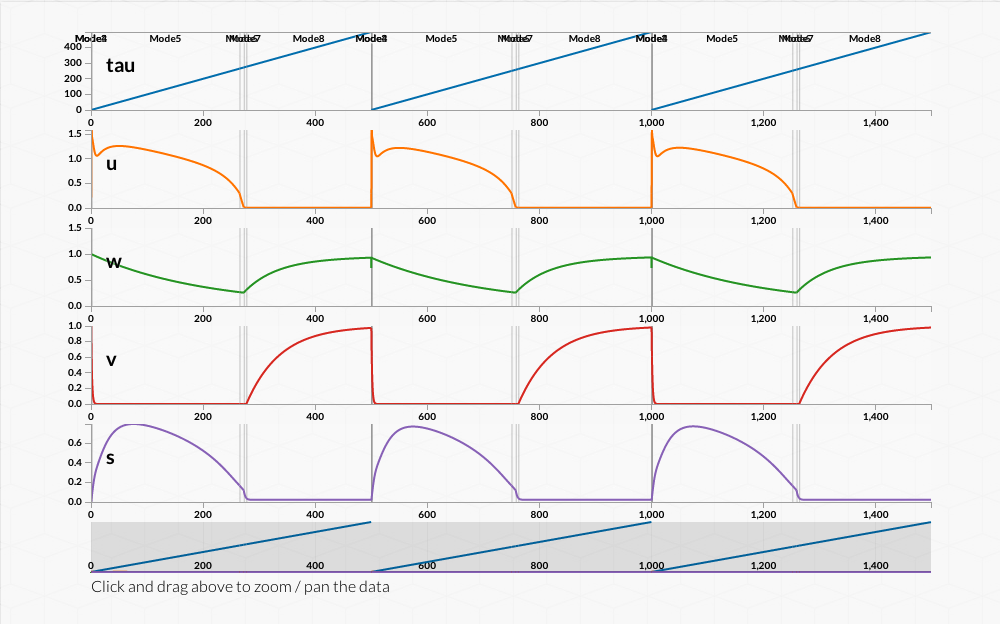
\includegraphics[width=\textwidth]{images/cardiac}
  \caption{Visualization of $\delta$-reachable trajectory for
    a cardiac-cell model.}
  \label{fig:viz}
\end{figure}


%%% Local Variables:
%%% mode: latex
%%% TeX-master: "main"
%%% End:
